	It is always important in the construction of  new algorithms to study  the global
discretization error and to give an estimation of the speed of convergence. 
Also we will study the stability of our numerical schemes. While convergence give us
information about behavior of a scheme on a fixed time interval letting the time-step small, the stability analysis
allow us to understand behavior of the approximation for a fixed step size when the time interval expands to infinity.
For simplicity, we study these properties for a one-dimensional autonomous SDE
\begin{equation}\label{eqn:autonomousSDE}
	dy(t)=fy(t))dt+g(y(t))dW(t).
\end{equation}
	As a fist step, we suppose that \Cref{ass:ClassicExisAndUniqueness} is fulfilled. But in \Cref{ch:Chapter5} 
we will work under a more general setting. Let us state the classic definitions of these concepts (see e.g. 
\cite{Kloeden1992}).
\subsection{Strong consistency and convergence}\label{sec3}
		As we mention above we  analyze the global discretization error and convergence. 
	 Here, they are	carried out with  the study of the properties of consistency and convergence, see
	\cite{Kloeden1992}. Here we state these concepts.
	\begin{dfn}\label{dfn:Consistency}
		A time discrete approximation $Y_n$ is strongly consistent if there is a nonnegative
		function $c=c(h)$ such that the following conditions hold for all fixed values $Y_n=y$,
		and $n=0,1,\dots, N$,
		\begin{enumerate}%[(i)]
			\item \label{eqn:DefConsitenceA}
		$\displaystyle \lim_{h\rightarrow 0} c(h)=0$,
			\item\label{eqn:DefConsitenceB}
		$\displaystyle \mathbb{E} \left(\left| \mathbb{E} \left(
				\frac{Y_{n+1}-Y_n}{h} \left|\mathcal{F}_{\tau_n}\right.
			\right)-F\left( Y_n \right)\right|^2 \right)\leq c(h),$
			\item \label{eqn:DefConsitenceC}
		$ \displaystyle  \mathbb{E} \left(\frac{1}{h} \
		\left|Y_{n+1}-Y_n-\mathbb{E}\left(Y_{n+1}-Y_n
		\left| \mathcal{F}_{\tau_n}\right.\right)-G\left(Y_n\right)
		\Delta B_n\right|^2 \right) \leq c(h)$.
		\end{enumerate}
	\end{dfn}
	On sake of clearness we define
	$\displaystyle n_t:= \max_{n=1 \ldots N}\{n: t_n\leq t\}$.
	\begin{dfn}
	A time discrete approximation $Y_n$ is strongly convergent  if for the end time $T$ is
	verified
	\begin{equation*}
		\lim_{h \rightarrow 0}
		\mathbb{E}\left| y(T)-Y_{n_T}\right|=0.
	\end{equation*}
	\end{dfn}

Now, we give a theorem that connects both concepts.
\begin{thm}[{\cite[Thm. 9.6.2]{Kloeden1992}}]\label{thm:ConsistencyConvergence}
	If $Y_n$ is a strongly consistent time discrete approximation maximum step $h$ of the
	solution  of the SDE \eqref{eqn:autonomousSDE} with $Y_0=y_0$. Then $Y_n$ converges
	strongly to the solution $y$.
\end{thm} 

\begin{definition}[order]
	A discrete approximation $Y_k$ \emph{converges strongly with order} $\delta$ at time $T$ if there exist a positive 
	constant $C$ independent of the step size $h$, such that
	\begin{equation}
	\EX{|y(T)-Y_{n_T}|} \leq C h^\delta.
	\end{equation}
	In addition, we say that a discrete approximation \emph{converges strongly} with order $\delta$ \emph{uniformly} on
	 time if
	\begin{equation}
	\EX{
		\sup_{1 \leq k\leq N}
		|y(t_k)-Y_k|
	}\leq C h^{\delta}.
	\end{equation}
\end{definition}


\subsection{Higham-Mao-Stuart proof convergence technique} \label{sec:HMS-Technique}
		Now we discuss a technique  reported  by  \citet*{Higham2002b} to prove strong convergence 
of stochastic numerical methods under non-globally Lipschitz conditions.
This kind of analysis is useful whenever moment bounds can be established for both, the EM scheme and 
other method that can be shown to be "close" to it. A vast amount of literature has been used this 
technique, some of these works are
\cite{Beyn2010, Guo2014, Hutzenthaler2015, Hutzenthaler2012a,Hutzenthaler2010,Lamba2007,Mao2013,Tretyakov2013}, among
others.

	To review this technique, we recall two conveniently versions for the continuous extension of the EM 
scheme,
\begin{align}\label{eqn:EMContinuousExtension}
	\overline{Y}(t)&:=
		Y_{\eta(t)} + (t-t_{\eta(t)}) f(Y_{\eta(t)}) + g(Y_{\eta(t)})(W(t)-W_{\eta(t)}),\\
		\eta(t)&:=
			 k, \text{ for } t\in[t_k,t_{k+1}), \notag
\end{align}
and
\begin{align}
		\overline{Y}(t)
		&:=
			Y_0 + \int_{0}^t f(Y_{\eta(s)})ds + 
			\int_0^tg(Y_{\eta(s)})dW(s). \notag \label{eqn:EMIntegralContinuousExtension}
\end{align}
So, with this notation we have $\overline{Y}(t_k)=Y_k$, see \Cref{fig:ContinuousExtension}.
%
\begin{figure}[h!]
	\centering
	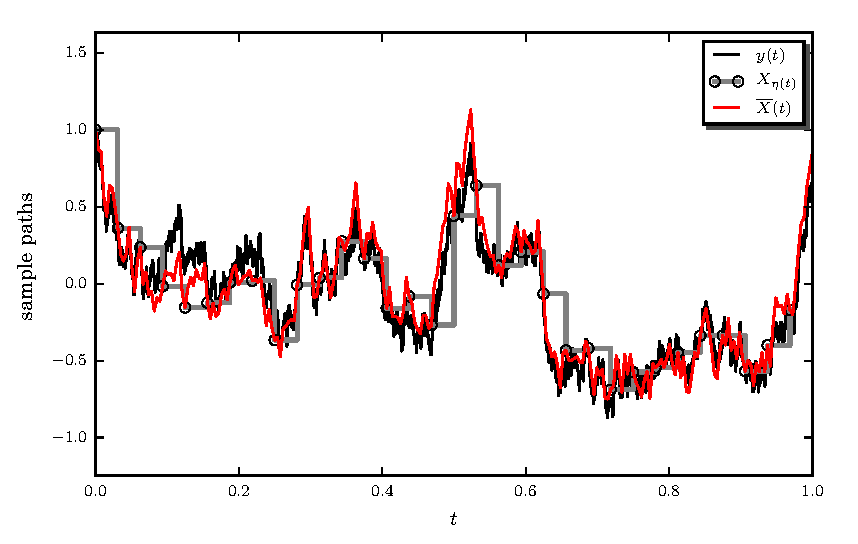
\includegraphics{papers/paperB/sections/ContinuousExtPy/ContinuousExtension.eps}
	\caption{
		The red line represents the continuous extension of the EM scheme. The continuous gray line is the 
		$Y_{\eta(t)}$ 
		process defined in \eqref{eqn:EulerMaruyama}.
	}
	\label{fig:ContinuousExtension}
\end{figure}
Using the continuous extension \eqref{eqn:EMContinuousExtension}
and the uniform mean square norm, the authors work with a stronger version of the ms-error%, which is given by 
$$
	\EX{\sup_{0\leq t \leq t}|y(t)-\overline{Y}(t)|^2}.
$$
%
Then, in  order to prove strong convergence of the EM method, the authors require the following assumptions.
\begin{assumption}\label{ass:HighamAssumption}
	For each $R>0$ there is a positive constant $C_R$, depending only on $R$, such that
	\begin{equation}\label{ass:LipschitzCondition}
		|f(x)-f(y)|^2 \vee |g(x)-g(y)|^2 \leq C_R|x-y|^2,
		\quad
		\forall x,y\in \R^d 
		\text{ with } |x|\vee |y|\leq R.
	\end{equation}
	And for some $p>2$, there is a constant $A$ such that
	\begin{equation}
		\EX{\sup_{0\leq t\leq T}|\overline{Y}(t)|^p}
		\vee
		\EX{\sup_{0\leq t\leq T}|y(t)|^p} \leq A.
	\end{equation}
\end{assumption}
In \cite{Higham2002b}, the authors prove that the \Cref{ass:HighamAssumption} is sufficient to ensure strong 
convergence for the EM scheme, namely 
\begin{thm}[
	{\cite[Thm 2.2]{Higham2002b}}
	]\label{thm:HighamMaoStuart}
	Under \Cref{ass:HighamAssumption}, the EM scheme \eqref{eqn:EulerMaruyama} with continuous extension
	\eqref{eqn:EMContinuousExtension}
	%\eqref{eqn:EMIntegralContinuousExtension} 
	satisfies
	\begin{equation}
		\lim_{h\to 0}
		\EX{\sup_{0\leq t\leq T}|\overline{Y}(t)-y(t)|^2}=0.
	\end{equation}
\end{thm}
	
	Applying this result, the authors prove the strong convergence of an implicit split-step variant of the EM, the
SSEM method. 
Their technique consist in proving each assertion of the following steps.
\begin{enumerate}[\bf{Step} 1:]
	\item
		\label{stp:EMCorrespondence}
		The SSEM for SDE \eqref{eqn:SDE1} is equivalent to the EM for the following conveniently SDE
		\begin{equation}\label{eqn:PerturbedHighamSDE}
			dy_h(t)= f_h(y_h(t))dt +g_h(y_h(t))dW(t).
		\end{equation}
	\item\label{stp:PerturbedSolution}
			The solution of the modified SDE \eqref{eqn:PerturbedHighamSDE} has bounded moments and it is 
			"close" to  $y$ the sense of the uniform mean square norm 
			$
				\EX{\sup_{0\leq t\leq T}|\cdot|^2}
			$.
	\item
	\label{stp:MethodBoundedMoments}
		Show that the SSEM method for the SDE \eqref{eqn:SDE1} has bounded moments.
	\item
		There is a continuous extension of the SSEM, $\overline{Z}(t)$, with bounded moments.
	\item
		Use the above steps and \Cref{thm:HighamMaoStuart} to conclude that
		\begin{equation}
			\lim_{h\to 0}
			\left\{
				\EX{\sup_{0\leq t\leq T}|y_h(t)-y(t)|^2}
			+
			\EX{\sup_{0\leq t\leq T}|\overline{Z}(t) -y_h(t)|^2}
			\right\}=0.
		\end{equation}
\end{enumerate}
In Chapter 4, we will use this technique.
% We will 
%use the same technique as these authors, that is, we will show that:
%\begin{inparaenum}[(a)]
%	\item
%		the underlying method corresponds to the EM for a perturbed SDE and
%	\item
%		all moments of the approximation are bounded.
%\end{inparaenum}
%
	Moreover, if we are interested in simulating the solution of the SDE \eqref{eqn:SDE} for large periods of time, 
	we need to use stable methods. We can interpret the stability of a numerical scheme, in some sense, as its
	capacity to preserve the  dynamical structure of the solution in that sense. Here we recall the topics that we will 
	work in the next chapter.
\subsection{Numerical Stability}
	With a numerical stability  one obtain  the step sizes for which a method reproduces  behavior of the solution 
	for a SDE. Therefore, it is important to know some qualitative  information  about the  solution, for example: if 
	all solution paths tend to a fixed point, or  if stay on a bounded set or reach an absorbent process.
	Usually the first step in this direction is a linear stability analysis. This study mimics the deterministic 
	context, which is based in the following steps:
	\begin{enumerate}[\bfseries{Step} 1:]
		\item 
			Expand in Taylor series around a fixed point the right hand side of a nonlinear ordinary differential 
			equation $x'(t) = f(t,x)$.
		\item
			Take a linear system with the Jacobian matrix of $f$ evaluated at the equilibrium
			$x'(t) = Ax(t)$.
		\item
			Diagonalize to decouples the linear system and study equations of the form
			$x'(t) = \lambda x(t), \lambda \in \C$.
	\end{enumerate}
	If all eigenvalues of $A$ are different from zero, then the  theorem of Hartman (see \cite{Hartman1960}) justifies 
	the use of this last equation  to study the behavior around a sufficient small neighborhood. So, one 
	seek conditions to assure that the numerical methods preserves the dynamics of underlying test. 
		
		In stochastic numerics, the linearization procedure is analogous  but here the linear SDE with multiplicative 
	noise is the benchmark test. The advantage of this linear SDE is that has the same unique fixed point as its 
	deterministic analogous, the origin \cite[]{Higham2000} .  Another benchmark equation is the linear SDE with 
	additive noise. However, for these model the concepts of numerical stability were unclear. The first works with 
	this test\cite{Hernandez1992,Milstein2004,Artemiev1997}, differs about the meaning of fixed point and stability. 
	Recently, the works of \citeauthor*{CruzCancino2010} \cite{CruzCancino2010} and \citeauthor*{Buckwar2011a} 
	\cite{Buckwar2011a} analyze the additive linear SDE using the theory of random dynamical systems, which in our 
	opinion clarifies this issue.
	
		Naturally the nonlinear case, is even more complex. Although  Lyapunov theory is the usual approach in 
	applications \cite{Khasminskii2011}, a more general novel approach based on the theory of random dynamical 
	systems \cite{Arnold1998} is a current topic of interest. In the following we provide this notions. 
		
\section*{Linear Stability}
	\subsection*{Multiplicative noise}
		Consider the scalar linear SDE
		\begin{equation}\label{eqn:SDEMultiplicativeNoise}
			dy(t)=\lambda y(t)dt+\xi y(t) dW(t) , \quad X_0=x_0,  \quad \lambda,\xi \in \C.
		\end{equation}
		The solutions of this SDE have the following property
		\begin{equation}\label{eqn:LinearMSEquivalence}
			\lim_{t\to\infty} \EX{|y(t)|^2} = 0 \Leftrightarrow \Re(\lambda) +\frac{1}{2} |\xi|^ 2 <0.
		\end{equation}
		A solution that satisfies  the previous limit  is a \emph{mean-square stable} solution. 
		Note that for $\xi = 0$ we have, $\Re(\lambda)<0$, which is the stability condition  for the deterministic case.
			
			Applying the EM method \eqref{eqn:EulerMaruyama} to \eqref{eqn:SDEMultiplicativeNoise}, we obtain
		\begin{equation}\label{eqn:MS-EMRecurrence}
			Y_{k+1} = \left(1 + h\lambda + \sqrt{h}\xi V_k\right)Y_k,
		\end{equation}
		where each $V_k$ is an independent $\calN(0,1)$ random variable. 
		In order to study the stability properties of the EM scheme, we must study
		the long time behavior of random variables of the form \eqref{eqn:MS-EMRecurrence}.
		Analogously, we will say that sequence \eqref{eqn:MS-EMRecurrence} is mean-square stable if 
		$
			\lim_{k \to  \infty}
				\EX{|Y_k|^2} = 0.
		$
		Note that the EM scheme depends upon the problem parameters $\lambda$ and  $\xi$, and the method
		parameter $h$. Then for a particular choice of parameters, we will say that the EM scheme is mean-square stable 
		if it produces a mean-square stable sequence. 
		Our interest lies in finding the parameter values for which the EM method is stable, and comparing results
		with the region $\Re(\lambda) + \frac{1}{2}|\xi|^2 < 0$ in \eqref{eqn:LinearMSEquivalence}
		for the underlying SDE (see \Cref{fig:StabilityPlotsMultiplicativeEM}). There is the following 
		result. 
		\begin{thm}
			Consider the EM method for the linear scalar SDE \eqref{eqn:SDEMultiplicativeNoise}. If the parameters 
			$\lambda$, $\xi$, and the step size $h$ satisfies
			$$
				\Re(\lambda) + \frac{1}{2}
				\left( |\xi|^2 + h|\lambda|^2\right) <0.
			$$
			Then the EM solution is \emph{mean square stable}.
		\end{thm}
		
		\begin{figure}[htb]
			\centering
			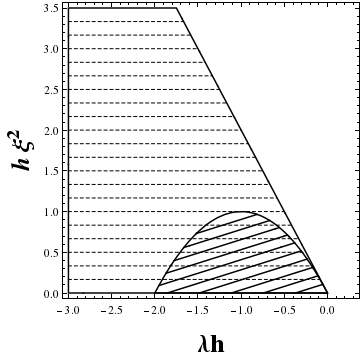
\includegraphics[scale=0.6]{Preliminaries/figures/StabilityPlotsMultiplicativeEM.png}
			\caption{Mean square regions of stability. The horizontal lines represents the stability region of
				SDE \eqref{eqn:SDEMultiplicativeNoise} and diagonal lines for the EM solution.
			}
			\label{fig:StabilityPlotsMultiplicativeEM}
		\end{figure}
			
	\subsection*{Additive noise}
	Here we study the additive linear SDE: 
	\begin{equation}\label{eqn:SDELinearAdditive}
		dy(t)=\lambda y(t)dt+ \xi  dW(t) , \qquad y_0=y_(t_0), \qquad \lambda, \xi \in \R.		
	\end{equation}
	where $\lambda$, $\xi \in \mathbb{C}$ and $X_{t_0}$ is the initial value of the process
	at time $t_0$. Equation \eqref{eqn:SDELinearAdditive}  has  the following  exact solution:
	\begin{equation}\label{eqn:OUProcess}
	y(t)=\exp(\lambda (t-t_0)) y(t_0)+\xi 
	\exp(\lambda t)\int\limits_{t_0}^{t}\exp(-\lambda s)dW(s), 
	\qquad t\geq t_0.
	\end{equation}
	The stochastic process $y(t)$ defined in \eqref{eqn:OUProcess} is known as 
	the {\it Ornstein-Uhlenbeck}'s (OU)  process. According to \cite{Hernandez1992},
	the OU process  is {\it asymptotically mean stable} if
	$ \lim_{t\to\infty}\m{y(t)}=0$ and is
	{\it  asymptotically  mean square stable} if
	$\displaystyle \lim_{t\to\infty}\ms{y(t)}=-\xi/2Re(\lambda)$. Both 
	limits are verified if $\lambda<0$. 
	Analogous stability properties are given for 
	stochastic  difference equations with additive noise \cite{SaiotoPreprint}. 
	Now, if we consider $\lambda<0$ then the OU solution \eqref{eqn:OUProcess} does 
	not convergence as $t$ tends to infinity but has the following pullback limit:
	\begin{equation}\label{eq4}
		\lim_{t_0\to-\infty} y(t)=\widehat{O}_t:=
		\exp(\lambda t)\int\limits_{-\infty}^{t}\exp(-\lambda s)dW(s), 
	\end{equation}
	$W(t)$  is now defined for all $t\in\mathbb{R}$, see
	\cite{Arnold1998, kloeden1999towards}. Furthermore, the process \eqref{eq4} is a
	stationary solution  of the additive linear SDE which attracts all other solutions in
	forward time and path-wise sense. Moreover, it is a finite process for all $t\geq
	T_{D(\omega)}$ ($\omega\in \Omega$) for  appropriate families $D(\omega)$ of bounded
	sets of initial conditions, see \cite{Robinson2002}. Therefore, 
	we can evaluate the numerical stability of a given stochastic method by examine if 
	this scheme reproduce the pullback asymptotic behavior.
	For example, the explicit EM scheme for \eqref{eqn:SDELinearAdditive}
	$$
		Y_{k+1} = (1+\lambda h) Y_n + \xi \Delta W_n,	
	$$
	given a initial value $Y_{k_0}$, has the form
	$$
		Y_{k+1} = (1+\lambda h)^{k-k_0} Y_{k_0}
			+\xi \sum_{j=k_0}^{k-1} (1+\lambda h)^{k-1-j} \Delta W_j.
	$$
	So, the path-wise pullback limit (taking $k_0 \to \infty$  with $k$ held fixed and $Y_{k_0} = Y_0$ for
	all $Y_{k_0}$ and constant time step $h$) exists, provided that $0 <h< 2/(- \lambda)$, $\lambda <0$, and is given
	by
	$$
		\widehat{O}_k^{(h)} := 
			\xi \sum_{j= -\infty}^k
				(1+\lambda h)^{1-k-j} \Delta W_j,
	$$
	for more details see the work of
	\citet*{Buckwar2011a}.
	
\section*{Non-Linear Stability}	
	Now we discuss the nonlinear case for multiplicative and additive noise. 
	\subsection*{Multiplicative Noise}
	We start with a notion of stability	which emulates the continuity respect to initial conditions of deterministic 
	ODEs.
	\begin{dfn}[\citeauthor{Baker2000a} {\cite{Baker2000a}}]\label{dfn:SNMS}
		Let $Y_n$ and $\widehat{Y}_n$ two different numerical recurrences  with
		corresponding initial process  $Y_0$ and $\widehat{Y}_0$. We shall say that a
		discrete time, $Y$ is \emph{numerically zero-stable in quadratic mean-square sense} if given
		$\epsilon >0$, there  are positive constants $h_0$ and $\delta=\delta(\epsilon,h_0)$
		such that for all $h\in(0,h_0)$ and positive integers $n \leq T/h$ whenever
		$\ms{Y_0-\widehat{Y}_0}<\delta$ then
		\begin {eqnarray}\label{eqn:SNMS}
		\rho_n :=
		\ms{Y_n-\widehat{Y}_{n}}<\epsilon .
	\end{eqnarray}
	If the method is stable and $\rho_n \to 0$ when $n\to \infty$, then the method is
	\emph{asymptotically zero-stable in the quadratic mean-square sense}.
\end{dfn}
Also, in \cite{Baker2000a} provides a result to characterizes this type of stability. Here we
enunciated it for the EM.
\begin{thm}[{\cite[Thm. 4 ]{Baker2000a}}]
	Let $C_1$, $C_2$ and $C_3$ generic positive constants which not depends on $h$ and $V$ a
	$\calN(0,1)$ random variable. 
	If the coefficients of  SDE \eqref{eqn:SDE} satisfies the estimates
	\begin{align*}
		\left|\EX{
			f(x) h +  g(x)\sqrt{h}V -
			\left(
				f(x') h + g(x')\sqrt{h}V
			\right)}	
		\right| 
		&\leq C_1h \left(|x - x'| \right), \\
		\EX{\left|
				hf(x)+g(x)\sqrt{h}V -
				\left(
				 f(x') h + g(x')\sqrt{h}V
				\right)	
			\right|^2}
			&\leq C_2 h \left(|x - x'| \right),
	\end{align*}
	then the EM method \eqref{eqn:EulerMaruyama} for \eqref{eqn:SDE} is zero-stable in the quadratic mean-square sense.
\end{thm}
%%%%%%%%%%%%%%%%%%%%%%%%%%%%%%%%%%%%%%%%%%%%%%%%%%%%%%%%%%%%%%%%%%%%%%%%%%%%%%%%%%%%%%%%%%
\subsection*{Additive noise}
		Nonlinear differential equations have more complex  dynamics than the linear case and
	the same  occurs for the finite difference equations. So,  \citeauthor*{Caraballo2006} in
	\cite{Caraballo2006}  extend the nonlinear stability theory of the deterministic
	numerical  analysis given in \cite{kloeden1999towards} to the stochastic
	case. They propose and justify the use of the following SDE as a test equation with additive noise:
	\begin{equation}\label{eqn:SemilinearSDE}
		dy(t)=\left(Ay(y)+f(y(t))\right)dt+\xi dW(t),
	\end{equation}
	where $A$ is a $d \times d$ stiff matrix and function $f : \R^d \to \R^d $ is a nonlinear and non-stiff function 
	that satisfies, a
	{\it contractive one-sided Lipschitz} condition with constant
	$L_1>0$
	\begin{equation}\label{cl}
		\langle
			u - v,f(u)-f(v)
		\rangle\leq
		-L_1|u-v|^2\qquad \forall u,v\in \mathbb{R}^d.
	\end{equation}
Also the authors give sufficient conditions to assure an asymptotically stable stochastic stationary solution
of \eqref{eqn:SemilinearSDE}. In this context they establish the following result for the stability of $\theta$-EM 
scheme.
\begin{thm}[{\cite[Thm. 3.1]{Buckwar2011a}}]
	Suppose that the drift coefficient satisfies a contractive one-sided Lipschitz condition, and that the vector field 
	f satisfies a globally Lipschitz condition . Then the $\theta$-EM scheme has a unique stochastic stationary 
	solution 
	which is pathwise asymptotically stable for all step sizes $h> 0$
	if
	$$
		(1-\theta) (|A|+L) <-\theta (\mu[A] - L_1),
		\qquad
		\mu[A] = \lim_{\delta \to 0^+} \frac{(|Id + \delta A|)}{\delta},
	$$
	where $L$ refers to the Lipschitz condition and $L_1$  the to contractive one-sided Lipschitz condition.
\end{thm}












The following chapter shows adaptations of these results for the construction of a new method, the Steklov method.
